\documentclass[11pt]{article}

% ---------- Packages ----------
\usepackage[utf8]{inputenc}
\usepackage[T1]{fontenc}
\usepackage{microtype}
\usepackage{geometry}
\geometry{letterpaper, margin=1in}
\usepackage{amsmath,amssymb,amsfonts}
\usepackage{amsthm}
\usepackage{algorithm}
\usepackage{algpseudocode}
\usepackage{booktabs}
\usepackage{multirow}
\usepackage{graphicx}
\usepackage{xcolor}
\usepackage{pgfplots}
\pgfplotsset{compat=1.18}
\usepackage{hyperref}
\hypersetup{colorlinks=true, linkcolor=blue, citecolor=blue, urlcolor=blue}
\usepackage[round]{natbib}
\usepackage{enumitem}
\usepackage{caption}
\usepackage{subcaption}

% ---------- Theorem environments ----------
\theoremstyle{plain}
\newtheorem{proposition}{Proposition}
\newtheorem{corollary}{Corollary}
\theoremstyle{definition}
\newtheorem{definition}{Definition}
\theoremstyle{remark}
\newtheorem{remark}{Remark}

% ---------- Title ----------
\title{HAC: Node-Level Hybrid Force--Graph Control and Smooth Handover Scheduling for Resilient UAV Swarm Connectivity Recovery}
\author{}
\date{}

\begin{document}
\maketitle

\begin{abstract}
Self-healing communication connectivity (SCC) for unmanned aerial vehicle (UAV) swarms requires rapidly reconnecting fractured subnetworks after partial node failures while preserving wide spatial coverage, yet pursuing either objective in isolation directly degrades the other. Recent hybrid frameworks such as R2C address this tension by combining intra-subnetwork virtual-force expansion with subnetwork-level multipartite graph convolution under a steep time-adaptive fusion schedule, bundling together several unisolated architectural choices. In this work, we formulate a three-axis taxonomy of the SCC design space spanning decision paradigm, spatial reasoning granularity, and trade-off scheduling, and systematically isolate each axis through five-seed controlled experiments. We propose Hybrid Adaptive Convolution (HAC), a lightweight node-level hybrid controller that fuses a parameter-free buffered virtual-force heuristic with a single global graph convolutional policy at the velocity level without subnetwork partitioning, convex-hull boundary extraction, or multipartite graph construction. Across random and uniform deployment scenarios under up to $80\%$ node failure, HAC under constant equal fusion weights outperforms purely heuristic, purely learned, and subnetwork-level rigid-translation baselines with substantially lower cross-seed variance and $1.5\times$ to $2.2\times$ faster execution, while retaining $88.4\%$ to $91.2\%$ of the coverage reported by R2C. Furthermore, we show that transplanting steep adaptive fusion schedules into simplified hybrid controllers severely degrades recovery robustness, whereas widening the transition window restores high recovery performance. Through theoretical analysis of neutral-zone velocity renormalization and a $3 \times 3$ decoupled training-versus-evaluation schedule study, we falsify the hypothesis that steep schedules corrupt policy learning during training and prove instead that premature inference-time handover extinguishes the heuristic link-retention barrier during long-horizon rollouts. Finally, granularity-substitution counter-experiments confirm that smooth scheduling rescues node-level policies but cannot rescue subnetwork-level rigid controllers that lack node-level actuation degrees of freedom.
\end{abstract}

\section{Introduction}
\label{sec:intro}

\subsection{Problem Context and Fundamental Trade-Off}
\textbf{Unmanned aerial vehicle (UAV) swarms deployed in contested or disaster-struck environments face recurring partial node failures that fracture communication topologies and degrade spatial coverage.} Wireless aerial networks provide rapid communication coverage in post-disaster relief, dynamic battlefields, and congested areas \citep{coletta2023auav,shi2025symmetry,wang2022task,wang2024angle}. During operation, internal hardware faults or external attacks can disable a subset of UAVs at any time \citep{wang2024survey,kurunathan2023machine}. When substantial node loss occurs, the surviving communication graph splits into multiple disconnected components, severely disrupting both multi-hop data routing and mission-area coverage \citep{li2023reinforcement,peng2022smarttro}. The self-healing communication connectivity (SCC) problem seeks a velocity control policy that repositions surviving UAVs so that the communication graph regains full connectivity as rapidly as possible while preserving maximal spatial coverage across the mission area.

\textbf{Accelerating topological reconnection and preserving spatial coverage impose directly opposing kinematic demands on surviving agents.} Pulling surviving UAVs inward toward a common center shortens reconnection time but contracts the covered footprint, whereas dispersing UAVs outward preserves area coverage at the risk of slowing or preventing link restoration. Managing this tension becomes increasingly difficult as the failure ratio approaches extreme regimes where surviving nodes are sparsely scattered across the arena.

\subsection{Limitations of Existing Paradigms}
\textbf{Purely heuristic recovery methods require no training data but scale poorly under severe, unstructured node failures.} Classical non-learning approaches either identify critical cut-vertices and trigger cascaded neighbor substitutions \citep{akkaya2009distributed,mi2015obstacle,zhang2024uavenabled} or guide surviving agents toward predefined rendezvous points using artificial potential fields \citep{joshi2012autonomous,shriwastav2018roundtable,chen2020sidr,wang2024apfcpp}. Because these methods rely on static topological assumptions and local interaction rules, they become brittle when large-scale failures isolate components beyond local sensing ranges \citep{tosun2024dpkcr}.

\textbf{Purely learned graph neural network (GNN) policies achieve rapid reconnection but suffer from spatial collapse.} Learning-based methods formulate SCC as a differentiable graph optimization or reinforcement learning problem \citep{mou2022resilient,peng2025prioritized,wang2025uav}. While GNN policies adapt effectively to diverse failure topologies, neighborhood message aggregation biases surviving UAVs to congregate around high-degree hubs, causing severe spatial clustering and coverage loss. Diffusion-based and differential-subgraph convolutions \citep{lin2024multihop,lin2025multihop} partially alleviate clustering by promoting multi-hop dispersion, yet they struggle to maintain stable layouts under extreme fragmentation and rarely enforce inter-agent spacing guarantees.

\subsection{Disentangling Hybrid Recovery Architecture and Scheduling}
\textbf{Recent divide-and-conquer hybrid frameworks achieve strong performance but bundle spatial granularity with steep adaptive scheduling.} To reconcile connectivity and coverage, \citet{peng2026r2c} introduced R2C, which combines a buffered virtual-force module for intra-subnetwork expansion (ISE) with a multipartite graph convolution module for inter-subnetwork translation (IST) governed by an adaptive weighted fusion (AWF) schedule. Because prior ablations toggle entire modules on or off, two fundamental design questions remain open regarding whether the learned branch must operate at subnetwork granularity with explicit convex-hull boundary extraction rather than globally at the node level, and whether adaptive fusion requires a steep temporal transition rather than a smooth or constant weighting.

\textbf{Controlled multi-seed ablations reveal that node-level hybrid fusion with fixed or smooth inference scheduling captures the vast majority of recovery performance without geometric partitioning.} We investigate these questions through Hybrid Adaptive Convolution (HAC), a streamlined architecture that fuses a parameter-free buffered virtual-force branch with a single global graph convolutional policy at the velocity level. Across five independent random seeds per configuration, our investigation yields four principal findings:
\begin{enumerate}[nosep]
  \item Fusing a global node-level learned branch with a parameter-free virtual-force heuristic under constant equal weights (HAC-Fixed) retains the vast majority of the coverage reported by complex multipartite architectures under extreme node failure while achieving near-complete recovery success, faster runtime execution, and substantially lower cross-seed variance than single-branch baselines.
  \item Directly porting a steep adaptive fusion schedule to this simplified architecture severely degrades recovery robustness under heavy node loss, whereas widening the transition slope (HAC-Smooth) restores high recovery performance across both random and uniform deployments.
  \item Decoupling training and evaluation schedules in a cross-evaluation matrix falsifies the hypothesis that steep schedules impair policy representation learning during training, proving instead that recovery collapse is an inference-time phenomenon caused by prematurely extinguishing the heuristic link-retention barrier over long evaluation horizons.
  \item Schedule smoothing rescues node-level hybrid control (HAC) but fails to rescue subnetwork-level rigid-translation hybrid control (HSC), cleanly separating an inference-time handover failure mode from an architectural expressiveness bottleneck.
\end{enumerate}

\subsection{Summary of Contributions}
The primary contributions of this paper are fourfold:
\begin{enumerate}[nosep]
  \item We formulate a three-axis taxonomy of the SCC design space spanning decision paradigm, spatial reasoning granularity, and trade-off strategy, positioning thirteen representative methods and isolating previously unexplored hybrid configurations.
  \item We propose HAC, a lightweight hybrid recovery architecture trained via a cardinality-invariant soft-minimum connectivity surrogate loss, and validate its resilience, computational efficiency, and variance-suppression properties across random and uniform deployments over five random seeds.
  \item We establish a theoretical and empirical diagnosis of hybrid fusion scheduling, combining formal analyses of link-retention barriers and neutral-zone velocity renormalization with a decoupled training-evaluation matrix that isolates inference-time handover instability from training-time curriculum effects.
  \item We provide a five-seed comparative analysis separating node-level versus subnetwork-level hybrid expressiveness, accompanied by open-source simulation code, training scripts, and complete multi-seed evaluation logs.
\end{enumerate}

The remainder of this paper is organized as follows. Section~\ref{sec:related-work} reviews related work, and Section~\ref{sec:prelim} formalizes the system model and design taxonomy. Section~\ref{sec:method} presents motivating single-branch failure modes and details the HAC framework. Section~\ref{sec:theory} provides our theoretical analysis of hybrid gating dynamics. Section~\ref{sec:results} reports the experimental setup, main five-seed benchmarks, and decoupled ablation studies. Section~\ref{sec:conclusion} discusses engineering implications, limitations, and conclusions.

\section{Related Work}
\label{sec:related-work}

\subsection{Non-Learning Self-Healing Methods}
\textbf{Critical-node compensation algorithms restore local links through cascaded neighbor movements but incur prohibitive coordination overhead as swarm scale grows.} Early self-healing protocols detect cut-vertices whose removal partitions the network and trigger sequential backup replacements \citep{abbasi2008movement,akkaya2009distributed,mi2015obstacle,zhang2024uavenabled}. While effective for isolated single-node faults, identifying critical nodes and coordinating multi-hop cascades scale poorly when simultaneous failures shatter the topology into numerous disjoint clusters.

\textbf{Rendezvous-point aggregation methods eliminate cut-vertex search but rely on static geometric rules that falter under unpredictable failure patterns.} Alternative heuristic schemes direct surviving UAVs or fractured subnetworks toward predetermined landmarks using Coulomb-inspired forces \citep{joshi2012autonomous}, round-table negotiation \citep{shriwastav2018roundtable}, or artificial potential fields \citep{chen2020sidr,wang2024apfcpp}. Although parameter-free and computationally lightweight, these hand-crafted rules lack global topological awareness and frequently stall in local equilibria or cause excessive coverage contraction under high failure ratios \citep{tosun2024dpkcr}.

\subsection{Learning-Based Self-Healing Methods}
\textbf{Graph neural network policies accelerate global reconnection but exhibit severe spatial collapse around high-degree nodes.} Posing connectivity recovery as a differentiable graph optimization problem enables end-to-end learning of coordinated trajectories \citep{karalias2020erdos,peng2025prioritized}. \citet{mou2022resilient} employ a relaxed GCN over virtual communication links, while \citet{guo2024intelligent} incorporate spatiotemporal multi-head attention. Despite fast convergence, standard message-passing schemes pull peripheral agents toward dense clusters, degrading coverage uniformity.

\textbf{Diffusion and differential-subgraph architectures improve spatial dispersion yet remain vulnerable to extreme topological fragmentation.} Recent works counter spatial collapse by introducing multi-hop diffusion convolutions \citep{lin2024multihop} or bipartite message passing over differential subgraphs \citep{lin2025multihop}. While these mechanisms encourage broader spatial spread, purely learned policies lack hard repulsive buffers to guarantee inter-agent spacing and exhibit high sensitivity to weight initialization when up to $80\%$ of the swarm is lost.

\subsection{Hybrid Heuristic--Learning Architectures and Positioning}
\label{sec:positioning}
\textbf{Hybrid recovery frameworks combine physical priors with learned graph representations to balance local spacing and global bridging.} \citet{peng2026r2c} proposed R2C, which pairs a buffered Hookean force field for intra-subnetwork expansion with a multipartite spectral GCN for inter-subnetwork translation using Quickhull boundary extraction \citep{barber1996quickhull} and asymmetric spectral filtering \citep{liu2025asymmetric}, blended via a sigmoid adaptive weighted fusion schedule \citep{elfwing2018sigmoid}. Elsewhere, \citet{li2025fast} combine distributed multi-agent reinforcement learning with artificial potential fields at the node level under fixed weighting, while \citet{wang2025uav} and related multi-robot coordination studies \citep{ye2022multiuav,mutzari2025heterogeneous,shi2025symmetry,kipf2016semi,zeng2023substructure} explore graph-based control without adaptive heuristic-learned velocity fusion.

\textbf{Our work isolates spatial reasoning granularity and schedule smoothness as independent design dimensions within the hybrid recovery paradigm.} Whereas prior studies evaluate hybrid modules as monolithic packages, we decompose the SCC design space along decision paradigm, spatial granularity, and trade-off scheduling. By holding the training objective and graph backbone fixed while systematically varying spatial granularity between node-level global control and subnetwork-level rigid translation and decoupling training-time versus inference-time fusion schedules, we identify the minimal architectural and dynamical conditions required for resilient recovery.

\section{System Model and Design Space Taxonomy}
\label{sec:prelim}

\subsection{UAV Swarm Network Model}
\textbf{The surviving UAV swarm is modeled as a time-varying proximity graph over a bounded planar mission area.} Following \citet{peng2026r2c}, at discrete time step $t$, the swarm forms a temporal graph $G_t = (V_t, E_t, P_t)$, where $V_t = \{v_{1,t}, \dots, v_{|V_t|,t}\}$ denotes the surviving UAVs, $E_t$ denotes the active communication links, and $P_t = \{\mathbf{p}_{1,t}, \dots, \mathbf{p}_{|V_t|,t}\}$ with $\mathbf{p}_{i,t} \in \mathcal{A} = [0, D_{\mathcal{A}}]^2 \subset \mathbb{R}^2$ represents their planar coordinates inside a square arena of side length $D_{\mathcal{A}}$. Let $\mathbf{A}_t$ be the binary adjacency matrix and $\mathbf{L}_t = \mathbf{D}_t - \mathbf{A}_t$ be the graph Laplacian. The number of connected components $C_t$ equals the algebraic multiplicity of the zero eigenvalue of $\mathbf{L}_t$, and global connectivity holds if and only if $C_t = 1$.

\textbf{Communication links and ground coverage follow Euclidean disk models governed by air-to-air path loss.} An undirected link $(v_i, v_j) \in E_t$ exists if and only if the inter-UAV distance $d_{ij,t} = \|\mathbf{p}_{i,t} - \mathbf{p}_{j,t}\|_2$ satisfies $d_{ij,t} \le R_c$, where $R_c$ is the communication range derived from free-space air-to-air channel models \citep{ma2019wideband,ni2024path,wang2025flight}. Each UAV covers a circular disk $\mathcal{C}_i(t)$ of radius $R_{\mathrm{cov}}$, yielding a collective swarm coverage ratio $C_{\mathrm{cov}}(t) = \bigl|\bigcup_{v_i \in V_t} \mathcal{C}_i(t)\bigr| / |\mathcal{A}|$.

\subsection{Optimization Objective and Kinematic Constraints}
\textbf{The self-healing connectivity recovery objective jointly penalizes reconnection delay and post-recovery coverage loss.} Let $t_1$ denote the failure onset step and $t_r = \min\{t \ge t_1 : C_t = 1\}$ denote the earliest step at which full connectivity is restored within evaluation horizon $T$, giving a normalized recovery time ratio $T_{\mathrm{rec}} = (t_r - t_1)/T$. We seek a velocity control policy $\hat{V}_t = \{\hat{\mathbf{v}}_{1,t}, \dots, \hat{\mathbf{v}}_{|V_t|,t}\}$ that minimizes the composite cost
\begin{equation}
  J_c = T_{\mathrm{rec}} + \bigl(1 - C_{\mathrm{cov}}(t_r)\bigr),
  \label{eq:objective}
\end{equation}
subject to four operational constraints: (C1) terminal connectivity $C_{t_r} = 1$; (C2) speed and arena bounds $\|\hat{\mathbf{v}}_{i,t}\|_2 \le \hat{v}_{\max}$ and $\mathbf{p}_{i,t} \in \mathcal{A}$; (C3) discrete-time Euler kinematics $\mathbf{p}_{i,t} = \mathbf{p}_{i,t_1} + \sum_{t_1 \le k < t} \Delta t \cdot \hat{\mathbf{v}}_{i,k}$; and (C4) link feasibility $d_{ij,t} \le R_c$ for all active intra-swarm transmissions. Minimizing $T_{\mathrm{rec}}$ requires inward convergence, whereas minimizing $1 - C_{\mathrm{cov}}(t_r)$ requires spatial dispersion.

\subsection{A Three-Axis Taxonomy of the Design Space}
\label{sec:taxonomy}
\textbf{Every self-healing recovery method can be categorized along three orthogonal design axes comprising decision paradigm, spatial granularity, and trade-off strategy.}
\begin{itemize}[nosep]
  \item \textbf{Axis 1 (Decision Paradigm):} Motion commands are generated by a \emph{heuristic} rule with zero learnable parameters, a \emph{learned} parametric network trained via data or differentiable simulation, or a \emph{hybrid} controller that explicitly fuses heuristic and learned outputs.
  \item \textbf{Axis 2 (Spatial Reasoning Granularity):} Control reasoning operates at the \emph{node-level} using local neighborhood states, the \emph{subnetwork-level} where each connected component acts as a rigid or coordinated unit, or the \emph{global-level} where all surviving agents exchange context across the entire arena.
  \item \textbf{Axis 3 (Connectivity--Coverage Trade-Off Strategy):} Competing objectives are balanced via a \emph{fixed} constant weight, a \emph{staged} sequential switch, or a continuous \emph{adaptive} schedule parameterized by time or topological state.
\end{itemize}
Table~\ref{tab:taxonomy} maps representative prior methods and our four experimental architectures (GAC, SAC, HAC, and HSC) into this $3 \times 3 \times 3$ combinatorial space.

\begin{table}[t]
\centering
\caption{Positioning of prior SCC methods and the architectures evaluated in this work within the $3\times3\times3$ design taxonomy.}
\label{tab:taxonomy}
\small
\begin{tabular}{@{}lllp{5.5cm}@{}}
\toprule
Paradigm & Granularity & Trade-off & Representative method(s) \\
\midrule
Heuristic & Node-level    & Fixed    & \citet{akkaya2009distributed,mi2015obstacle,wang2024apfcpp} \\
Heuristic & Subnetwork    & Fixed    & \citet{chen2020sidr} \\
Heuristic & Global        & Fixed    & \citet{lin2025multihop} \\
Heuristic & Global        & Staged   & HERO \citep{mi2011hero} \\
Learned   & Node-level    & Fixed    & \citet{mou2022resilient}; \textbf{GAC} (this work) \\
Learned   & Subnetwork    & Fixed    & \citet{lin2024multihop}; \textbf{SAC} (this work) \\
Learned   & Global        & Fixed    & \citet{guo2024intelligent} \\
Hybrid    & Node-level    & Fixed    & \citet{li2025fast} \\
Hybrid    & Node+Subnet   & Adaptive & R2C (ISE+IST+AWF) \citep{peng2026r2c} \\
\textbf{Hybrid} & \textbf{Global} & \textbf{Fixed / Adaptive} & \textbf{HAC (this work)} \\
\textbf{Hybrid} & \textbf{Subnetwork} & \textbf{Fixed / Adaptive} & \textbf{HSC (this work)} \\
\bottomrule
\end{tabular}
\end{table}

\section{Hybrid Adaptive Convolution (HAC) Framework}
\label{sec:method}
\label{sec:motivating}

\subsection{Complementary Failure Modes of Single-Branch Baselines}
\label{sec:gac}
\label{sec:sac}
\label{sec:takeaway}
\textbf{Purely learned global node-level policies (GAC) and subnetwork-level rigid-translation policies (SAC) fail in opposite, complementary ways that directly motivate node-level hybridization.} Before introducing HAC, we isolate two single-branch learned baselines that share identical loss functions and $4$-layer GCN backbones but operate at opposite spatial granularities:
\begin{itemize}[nosep]
  \item \textbf{Global Node-Level Learned Policy (GAC):} GAC constructs a symmetric $k$-nearest-neighbor ($k$-NN) graph over the Euclidean coordinates of all surviving UAVs regardless of communication range $R_c$, allowing message passing across disconnected components to output per-node 2D velocities (corresponding to the pure learned branch with $w_T=1, w_E=0$). As shown in Table~\ref{tab:gac-sac-random}, GAC's recovery success rate under random deployment drops from $45.6 \pm 2.9$ out of $50$ trials at $20\%$ failure to $8.6 \pm 3.3$ at $80\%$ failure, accompanied by an elevated average node degree ($\mathrm{AND}$ reaching $9.07 \pm 0.44$ at $20\%$ and $10.12 \pm 0.33$ at $40\%$ failure) that reflects severe spatial clustering around high-degree nodes.
  \item \textbf{Subnetwork-Level Rigid Translation (SAC):} SAC partitions surviving UAVs into connected components under $R_c$, pools each component into its centroid position and relative size, and applies the same $4$-layer GCN over a $k$-NN graph of component centroids to predict a single rigid 2D translation vector shared by all members of each subnetwork. Table~\ref{tab:gac-sac-random} shows that SAC maintains a low, uniform node degree ($\mathrm{AND} = 6.71 \pm 0.09$ at $20\%$ failure and $5.32 \pm 0.18$ at $40\%$ failure), eliminating intra-cluster collapse. However, its recovery success rate drops to $29.4 \pm 3.4$ at $20\%$ failure, $8.8 \pm 1.9$ at $40\%$ failure, and collapses deterministically to $0.0 \pm 0.0$ out of $50$ at both $60\%$ and $80\%$ failure across all five seeds.
\end{itemize}
GAC retains full $2|V_t|$ spatial degrees of freedom to bridge fragmented clusters but lacks a short-range repulsive mechanism to prevent over-concentration, whereas SAC preserves internal spacing by freezing relative intra-component positions but loses the ability to deform components toward multiple scattered targets. This complementarity motivates fusing a parameter-free local virtual-force field with a node-level global GCN policy.

\begin{table}[t]
\centering
\caption{Motivating single-branch comparison under random deployment (mean $\pm$ std over 5 seeds, 50 trials per seed). GAC (global node-level learned-only) suffers from spatial clustering (elevated AND), whereas SAC (subnetwork rigid translation) avoids clustering but collapses deterministically at $60\%$--$80\%$ failure.}
\label{tab:gac-sac-random}
\small
\begin{tabular}{@{}lcccc@{}}
\toprule
Failure & \multicolumn{2}{c}{GAC (global node-level)} & \multicolumn{2}{c}{SAC (subnetwork rigid)} \\
\cmidrule(lr){2-3} \cmidrule(lr){4-5}
Rate & AND & Success/50 $\uparrow$ & AND & Success/50 $\uparrow$ \\
\midrule
20\% & $9.073 \pm 0.442$  & $45.6 \pm 2.9$ & $6.713 \pm 0.091$ & $29.4 \pm 3.4$ \\
40\% & $10.121 \pm 0.331$ & $37.8 \pm 3.5$ & $5.324 \pm 0.183$ & $8.8  \pm 1.9$ \\
60\% & $9.267 \pm 0.460$  & $26.4 \pm 2.8$ & n/a               & $0.0  \pm 0.0$ \\
80\% & $5.104 \pm 0.334$  & $8.6  \pm 3.3$ & n/a               & $0.0  \pm 0.0$ \\
\bottomrule
\end{tabular}
\end{table}

\subsection{Heuristic Branch: Buffered Three-Zone Virtual-Force Field}
\label{sec:heuristic-branch}
\textbf{The heuristic branch regulates local inter-UAV spacing and arena containment through a parameter-free three-zone potential field.} Adopting the buffered virtual-spring formulation \citep{rychlewski1984hooke,peng2026r2c}, we partition the communication disk $(0, R_c]$ around an equilibrium neutral zone $[d_l, d_u] = [0.8 R_c, 0.9 R_c]$. The pairwise virtual force exerted on UAV $v_i$ by a communicating neighbor $v_j \in \mathcal{N}_i = \{v_j \in V_t : 0 < d_{ij,t} \le R_c\}$ is defined as
\begin{equation}
  \mathbf{F}'_{ij,t} =
  \begin{cases}
    -\exp\!\left(-\alpha \cdot \dfrac{d_{ij,t}}{d_l}\right) \mathbf{u}_{ij,t}, & 0 \le d_{ij,t} < d_l \\[6pt]
    \mathbf{0}, & d_l \le d_{ij,t} \le d_u \\[4pt]
    \exp\!\left(-\beta \cdot \dfrac{R_c - d_{ij,t}}{R_c - d_u}\right) \mathbf{u}_{ij,t}, & d_u < d_{ij,t} \le R_c,
  \end{cases}
  \label{eq:heuristic-force}
\end{equation}
where $\mathbf{u}_{ij,t} = (\mathbf{p}_{j,t} - \mathbf{p}_{i,t}) / d_{ij,t}$ is the unit direction vector from $v_i$ to $v_j$, and $\alpha = \beta = 0.01$ govern the exponential decay rates in the repulsive zone $[0, d_l)$ and attractive buffer zone $(d_u, R_c]$. To prevent agents from exiting the mission area $\mathcal{A}$, any UAV within distance $d_{i,k} < d_e = 0.15 R_c$ of boundary edge $k \in \mathcal{B} = \{\text{left, right, bottom, top}\}$ experiences an inward normal repulsion $\mathbf{F}''_{i,t} = \sum_{k \in \mathcal{B}} \exp(-\delta \cdot d_{i,k})\,\mathbf{n}_k$ with $\delta = 0.01$. Summing $\mathbf{F}_{i,t} = \sum_{j \in \mathcal{N}_i} \mathbf{F}'_{ij,t} + \mathbf{F}''_{i,t}$ and normalizing yields the heuristic velocity command $\mathbf{v}'_{i,t} = \hat{v}_{\max} \cdot \mathbf{F}_{i,t} / (\|\mathbf{F}_{i,t}\|_2 + \epsilon)$. Because Eq.~\eqref{eq:heuristic-force} contains no trainable weights, $\mathbf{v}'_{i,t}$ provides an invariant physical anchor throughout both training and inference.

\subsection{Learned Branch and Velocity-Level Adaptive Fusion}
\label{sec:learned-branch}
\label{sec:fusion}
\textbf{The learned branch propagates topological context across disconnected components via a global $k$-NN graph convolutional network without boundary-hull extraction.} At each step $t$, we construct a symmetric $k$-NN graph ($k=8$) over the Euclidean coordinates of all surviving UAVs $V_t$. Each node $v_i$ receives a $3$-dimensional input feature vector comprising its normalized planar coordinates and its normalized $k$-NN degree. This feature representation passes through an $L=4$ layer GCN with hidden dimension $128$ and ReLU activations, followed by a two-layer MLP head with $\tanh$ activation scaled by $\hat{v}_{\max}$ to produce the learned velocity vector $\mathbf{v}''_{i,t}$.

\textbf{Velocity-level fusion combines heuristic and learned commands through a horizon-normalized sigmoid schedule followed by unit-speed renormalization.} To govern the temporal handover from heuristic expansion to learned global translation over an active rollout horizon $H \in \{T_{\mathrm{train}}, T\}$, we define the time-dependent gating weights
\begin{equation}
  w_T(t; H) = \frac{1}{1 + \exp\bigl(-k \cdot (t/H - s_0)\bigr)}, \qquad w_E(t; H) = 1 - w_T(t; H),
  \label{eq:awf-schedule}
\end{equation}
where $k > 0$ controls transition steepness and $s_0 \in (0, 1)$ specifies the crossover midpoint relative to the active horizon $H$ ($H = T_{\mathrm{train}}$ during training and $H = T$ during evaluation). The executed velocity command $\hat{\mathbf{v}}_{i,t}$ is obtained by renormalizing the weighted sum:
\begin{equation}
  \hat{\mathbf{v}}_{i,t} = \hat{v}_{\max} \cdot
  \frac{w_E(t; H)\,\mathbf{v}'_{i,t} + w_T(t; H)\,\mathbf{v}''_{i,t}}
       {\left\| w_E(t; H)\,\mathbf{v}'_{i,t} + w_T(t; H)\,\mathbf{v}''_{i,t} \right\|_2 + \epsilon}.
  \label{eq:fusion}
\end{equation}
We evaluate three primary configurations of Eq.~\eqref{eq:fusion}: \textbf{HAC-Fixed}, which sets constant equal weights $w_E = w_T = 0.5$; \textbf{HAC-Adaptive} (including \textbf{HAC-Smooth} with $k=5, s_0=0.7$ and \textbf{HAC-Steep} with $k=30, s_0=0.125$), which varies $(k, s_0)$ in Eq.~\eqref{eq:awf-schedule}; and the single-branch baselines \textbf{GAC} ($w_T = 1, w_E = 0$) and \textbf{Heuristic-only} ($w_E = 1, w_T = 0$).

\subsection{Cardinality-Invariant Training Objective and Algorithms}
\label{sec:objective}
\textbf{A cardinality-invariant soft-minimum connectivity surrogate eliminates component-size bias during differentiable multi-step rollout training.} Because the discrete component count $C_t$ is non-differentiable, we supervise inter-component bridging using a smooth soft-minimum distance surrogate over every pair of currently disconnected components $S_i, S_j$:
\begin{equation}
  \mathcal{L}_{\mathrm{conn}}^{(i,j)} =
  -\tau \left( \log \sum_{\substack{u \in S_i \\ v \in S_j}}
  \exp\!\left(-\frac{d_{uv}}{\tau}\right) - \log(n_i n_j) \right),
  \label{eq:conn-loss}
\end{equation}
averaged over all disconnected component pairs, where $n_i = |S_i|$, $n_j = |S_j|$, and $\tau > 0$ is a temperature parameter. Standard log-sum-exp soft-minimum estimators omit the $-\log(n_i n_j)$ correction, introducing an additive distortion of $-\tau \log(n_i n_j)$ that systematically under-penalizes large components and yields spuriously negative loss values (verified numerically in Appendix~\ref{app:deviations}). Including $-\log(n_i n_j)$ ensures exact cardinality invariance so that isolated singletons receive gradient magnitudes consistent with large subnetworks.

\textbf{Spatial coverage and movement efficiency are supervised jointly through differentiable grid-coverage and displacement regularizers.} We approximate area coverage over a uniform grid $G \subset \mathcal{A}$ via $\mathcal{L}_{\mathrm{cov}} = \frac{1}{|G|} \sum_{\mathbf{g} \in G} \bigl(1 - \sigma\bigl((R_{\mathrm{cov}} - \min_i \|\mathbf{g} - \mathbf{p}_i\|_2)/\tau'\bigr)\bigr)$ and penalize excessive control effort via $\mathcal{L}_{\mathrm{move}} = \frac{1}{|V_t|}\sum_i \|\mathbf{p}_{i,t+1} - \mathbf{p}_{i,t}\|_2$. Throughout training, connectivity and coverage losses receive equal static weights of $0.5$, ensuring that all temporal trade-offs occur strictly at the velocity fusion layer in Eq.~\eqref{eq:fusion}. Algorithms~\ref{alg:hac-train} and~\ref{alg:hac-deploy} summarize end-to-end differentiable rollout training and closed-loop deployment.

\begin{algorithm}[t]
\caption{HAC Differentiable Rollout Training (One Epoch)}
\label{alg:hac-train}
\begin{algorithmic}[1]
\Require Learned policy $\pi_\theta$, training rollout length $T_{\mathrm{train}}$, training schedule $w_T^{\mathrm{train}}(\cdot; T_{\mathrm{train}})$
\State Sample failure ratio $r \sim \{0.2, 0.4, 0.6, 0.8\}$, initialize positions $\mathbf{P}_0$, and remove failed nodes
\State $\mathcal{L}_{\text{total}} \gets 0$
\For{$t = 0, \dots, T_{\mathrm{train}}-1$}
  \State Identify connected components $\{S_m\}$ of $\mathbf{P}_t$ under communication range $R_c$
  \State Compute heuristic velocities $\mathbf{v}'$ via Eq.~\eqref{eq:heuristic-force} \Comment{detached, zero trainable parameters}
  \State Construct global $k$-NN graph over $\mathbf{P}_t$ and evaluate $\mathbf{v}'' \gets \pi_\theta(\mathbf{P}_t)$ \Comment{learned branch}
  \State Evaluate gating weights $w_T \gets w_T^{\mathrm{train}}(t; T_{\mathrm{train}})$ and $w_E \gets 1 - w_T$
  \State Fuse velocities $\hat{\mathbf{v}} \gets \text{Fuse}(\mathbf{v}', \mathbf{v}'', w_E, w_T)$ via Eq.~\eqref{eq:fusion}
  \State Update positions $\mathbf{P}_{t+1} \gets \text{clip}(\mathbf{P}_t + \Delta t \cdot \hat{\mathbf{v}}, \; 0, \; D_{\mathcal{A}})$
  \State $\mathcal{L}_{\text{total}} \gets \mathcal{L}_{\text{total}} + 0.5\,\mathcal{L}_{\mathrm{conn}}(\mathbf{P}_{t+1}) + 0.5\,\mathcal{L}_{\mathrm{cov}}(\mathbf{P}_{t+1}) + \lambda\,\mathcal{L}_{\mathrm{move}}$
\EndFor
\State Backpropagate $\mathcal{L}_{\text{total}} / T_{\mathrm{train}}$ through $\pi_\theta$ and update $\theta$ via Adam with gradient clipping
\end{algorithmic}
\end{algorithm}

\begin{algorithm}[t]
\caption{HAC Inference Deployment Rollout}
\label{alg:hac-deploy}
\begin{algorithmic}[1]
\Require Trained policy $\pi_\theta$, evaluation horizon $T$, evaluation schedule $w_T^{\mathrm{eval}}(\cdot; T)$
\For{$t = 0, \dots, T-1$}
  \If{$C_t = 1$ (swarm is fully connected)} \textbf{return} success, recovery step $t$
  \EndIf
  \State Compute heuristic velocities $\mathbf{v}'$ via Eq.~\eqref{eq:heuristic-force}
  \State Evaluate learned velocities $\mathbf{v}'' \gets \pi_\theta(\mathbf{P}_t)$ \Comment{no gradient computation}
  \State Fuse velocities $\hat{\mathbf{v}} \gets \text{Fuse}(\mathbf{v}', \mathbf{v}'', 1-w_T^{\mathrm{eval}}(t; T), w_T^{\mathrm{eval}}(t; T))$ via Eq.~\eqref{eq:fusion}
  \State Update positions $\mathbf{P}_{t+1} \gets \text{clip}(\mathbf{P}_t + \Delta t \cdot \hat{\mathbf{v}}, \; 0, \; D_{\mathcal{A}})$
\EndFor
\State \textbf{return} failure (horizon $T$ exhausted)
\end{algorithmic}
\end{algorithm}

\section{Theoretical Analysis of Hybrid Gating Dynamics}
\label{sec:theory}

We now establish two structural properties of the velocity-level hybrid controller that explain why maintaining a non-vanishing heuristic weight $w_E(t; H)$ alongside a non-vanishing learned weight $w_T(t; H)$ is essential for long-horizon recovery, and why steep gating transitions trigger collapse.

\subsection{Link-Retention Barrier in the Attractive Buffer Zone}
\label{sec:monotonicity}

\begin{proposition}[Link-retention barrier in the attractive buffer zone]
\label{prop:monotonicity}
Let $v_i, v_j$ be two connected UAVs occupying the attractive buffer zone $d_u < d_{ij,t} \le R_c$ of Eq.~\eqref{eq:heuristic-force}, and suppose no external repulsive or boundary force acts on $v_i$ or $v_j$. Then, for any step size $0 < \Delta t < d_{ij,t} / (2\hat{v}_{\max})$, executing the heuristic branch alone ($w_E = 1, w_T = 0$ in Eq.~\eqref{eq:fusion}) strictly decreases their inter-UAV distance according to $d_{ij,t+\Delta t} = d_{ij,t} - 2\Delta t\,\hat{v}_{\max} < R_c$, thereby guaranteeing that the existing communication link $(v_i, v_j) \in E_t$ cannot break at step $t + \Delta t$.
\end{proposition}

\begin{proof}
By Eq.~\eqref{eq:heuristic-force}, the pairwise force on $v_i$ from $v_j$ within $d_u < d_{ij,t} \le R_c$ is $\mathbf{F}'_{ij,t} = \exp\bigl(-\beta (R_c - d_{ij,t})/(R_c-d_u)\bigr) \mathbf{u}_{ij,t}$ pointing from $v_i$ toward $v_j$. By symmetry, $\mathbf{F}'_{ji,t} = -\mathbf{F}'_{ij,t}$ points from $v_j$ toward $v_i$ with equal magnitude. Under the isolation assumption, $\mathbf{F}_{i,t} = \mathbf{F}'_{ij,t}$ and $\mathbf{F}_{j,t} = -\mathbf{F}'_{ij,t}$, which after unit-speed normalization yields $\mathbf{v}'_{i,t} = \hat{v}_{\max}\,\mathbf{u}_{ij,t}$ and $\mathbf{v}'_{j,t} = -\hat{v}_{\max}\,\mathbf{u}_{ij,t}$. Applying the one-step Euler update gives $d_{ij,t+\Delta t} = \|\mathbf{p}_{i,t} + \Delta t\,\mathbf{v}'_{i,t} - \mathbf{p}_{j,t} - \Delta t\,\mathbf{v}'_{j,t}\|_2 = \|(\mathbf{p}_{i,t} - \mathbf{p}_{j,t}) + 2\Delta t\, \hat{v}_{\max}\, \mathbf{u}_{ij,t}\|_2$. Substituting $\mathbf{p}_{i,t}-\mathbf{p}_{j,t} = -d_{ij,t}\,\mathbf{u}_{ij,t}$ yields $d_{ij,t+\Delta t} = |d_{ij,t} - 2\Delta t\, \hat{v}_{\max}| = d_{ij,t} - 2\Delta t\,\hat{v}_{\max} < d_{ij,t} \le R_c$ for all $0 < \Delta t < d_{ij,t}/(2\hat{v}_{\max})$.
\end{proof}

\subsection{State-Triggered Priority via Neutral-Zone Renormalization}
\label{sec:neutral-zone}

\textbf{Combining the three-zone potential field with unit-speed renormalization creates an automatic state-triggered switching mechanism between global translation and local boundary protection.} A critical question is why HAC-Smooth ($k=5, s_0=0.7$), which assigns $w_E(t; H) > 0.5$ for the first $70\%$ of the horizon, still achieves rapid global reconnection ($\mathrm{REC} = 0.684$), whereas Steep Mid ($k=30, s_0=0.5$) stalls ($\mathrm{REC} = 0.855$) and collapses to $5.2/50$ successes. Proposition~\ref{prop:neutral-renorm} resolves this paradox.

\begin{proposition}[State-triggered priority under non-vanishing smooth gating]
\label{prop:neutral-renorm}
Suppose the gating weights in Eq.~\eqref{eq:fusion} satisfy the non-vanishing dominance condition $\epsilon \ll w_T(t; H)\|\mathbf{v}''_{i,t}\|_2$ and $w_E(t; H) > w_T(t; H)$ with $\|\mathbf{v}''_{i,t}\|_2 \le \hat{v}_{\max}$. Then at any time step $t$, the fused velocity command $\hat{\mathbf{v}}_{i,t}$ operates in two state-triggered regimes:
\begin{enumerate}[nosep]
  \item \textbf{Full-speed global translation inside the neutral zone:} If agent $v_i$ resides strictly inside the interior equilibrium zone ($d_l \le d_{ij,t} \le d_u$ for all $v_j \in \mathcal{N}_i$ and $d_{i,k} \ge d_e$), then $\mathbf{F}_{i,t} = \mathbf{0}$ and $\mathbf{v}'_{i,t} = \mathbf{0}$, so Eq.~\eqref{eq:fusion} simplifies to
  \begin{equation}
    \hat{\mathbf{v}}_{i,t} = \hat{v}_{\max} \cdot \frac{w_T(t; H)\,\mathbf{v}''_{i,t}}{w_T(t; H)\|\mathbf{v}''_{i,t}\|_2 + \epsilon} \approx \hat{v}_{\max} \frac{\mathbf{v}''_{i,t}}{\|\mathbf{v}''_{i,t}\|_2},
    \label{eq:neutral-amplification}
  \end{equation}
  driving $v_i$ at maximum speed $\hat{v}_{\max}$ along the learned global direction regardless of how small $w_T(t; H)$ is relative to $w_E(t; H)$.
  \item \textbf{Heuristic barrier priority outside the neutral zone:} Whenever any link enters the attractive buffer zone $(d_u, R_c]$ or repulsive zone $[0, d_l)$ such that $\|\mathbf{v}'_{i,t}\|_2 \approx \hat{v}_{\max}$, the inner product between the fused velocity $\hat{\mathbf{v}}_{i,t}$ and the heuristic restoration direction $\mathbf{v}'_{i,t}$ is strictly positive:
  \begin{equation}
    \langle \hat{\mathbf{v}}_{i,t}, \mathbf{v}'_{i,t} \rangle \ge \hat{v}_{\max}^2 \cdot \frac{w_E(t; H) - w_T(t; H)}{w_E(t; H) + w_T(t; H) + \epsilon/\hat{v}_{\max}} > 0,
  \end{equation}
  guaranteeing that the learned branch cannot reverse the heuristic link-retention or anti-collision direction.
\end{enumerate}
\end{proposition}

\begin{proof}
In Regime 1, substituting $\mathbf{v}'_{i,t} = \mathbf{0}$ into Eq.~\eqref{eq:fusion} factors $w_T(t; H) > 0$ out of both numerator and denominator; since $w_T(t; H)\|\mathbf{v}''_{i,t}\|_2 \gg \epsilon$, the scalar weight $w_T(t; H)$ cancels out, yielding unit-speed motion along $\mathbf{v}''_{i,t}$. In Regime 2, using $\|\mathbf{v}'_{i,t}\|_2 = \hat{v}_{\max}$, $\|\mathbf{v}''_{i,t}\|_2 \le \hat{v}_{\max}$, and the Cauchy--Schwarz inequality $\langle \mathbf{v}'_{i,t}, \mathbf{v}''_{i,t} \rangle \ge -\hat{v}_{\max}^2$, the numerator of $\langle \hat{\mathbf{v}}_{i,t}, \mathbf{v}'_{i,t} \rangle$ is bounded below by $\hat{v}_{\max}\bigl(w_E\|\mathbf{v}'_{i,t}\|_2^2 + w_T\langle \mathbf{v}''_{i,t}, \mathbf{v}'_{i,t}\rangle\bigr) \ge \hat{v}_{\max}^3(w_E - w_T) > 0$, while the denominator is bounded above by $w_E\hat{v}_{\max} + w_T\hat{v}_{\max} + \epsilon$.
\end{proof}

\begin{remark}[Why Smooth Late $(5, 0.7)$ succeeds while Steep Early $(30, 0.125)$ and Steep Mid $(30, 0.5)$ fail]
Proposition~\ref{prop:neutral-renorm} explains the entire schedule sweep:
\begin{itemize}[nosep]
  \item Under \textbf{HAC-Smooth $(k=5, s_0=0.7)$}, the initial weight is $w_T(0; H) = \sigma(-3.5) \approx 0.029 \gg \epsilon$, while $w_E(t; H) > w_T(t; H)$ holds for $70\%$ of the horizon. Both conditions of Proposition~\ref{prop:neutral-renorm} are satisfied simultaneously: equilibrated interior nodes translate at full speed $\hat{v}_{\max}$ toward distant components from $t=0$ onward, while boundary nodes retain strict link-retention protection ($w_E > w_T$) across the majority of the rollout.
  \item Under \textbf{Steep Early $(k=30, s_0=0.125)$}, $w_E(t; H)$ drops below $w_T(t; H)$ after only $12.5\%$ of the horizon ($t = 50$ steps) and vanishes ($w_E < 10^{-3}$) by $t = 142$, violating Condition 2 of Proposition~\ref{prop:neutral-renorm} for over $80\%$ of the $400$-step rollout and causing severe spatial clustering and link tearing.
  \item Under \textbf{Steep Mid $(k=30, s_0=0.5)$}, the initial weight is $w_T(0; H) = \sigma(-15) \approx 3.06 \times 10^{-7}$, which is microscopic during the first $35\%$ of the episode (violating Condition 1 when $\mathbf{v}'_{i,t} \approx \mathbf{0}$ or under tiny residual forces), wasting nearly half the horizon before abruptly flipping to $w_E(t; H) \to 0$ after $t = 200$ (violating Condition 2).
\end{itemize}
\end{remark}

\subsection{Autonomy Exposure and Decoupled Schedule Testability}
\label{sec:curriculum}
\label{sec:prediction}
\textbf{A competing training-time hypothesis posits that steep schedules degrade policy learning by inflating autonomy exposure during differentiable rollouts, a claim that can be directly falsified by decoupling training and evaluation schedules.} Because $\pi_\theta$ is trained end-to-end through Eq.~\eqref{eq:fusion} in Algorithm~\ref{alg:hac-train}, the schedule profile $w_T(t; H)$ determines the fraction of rollout steps in which the learned branch holds majority control:
\begin{equation}
  \mathrm{AE}_H(k, s_0; \tau) = \frac{1}{H} \Bigl|
  \bigl\{\, t \in \{0,\dots,H-1\} : w_T(t; H) > \tau \,\bigr\}
  \Bigr|.
\end{equation}
For $\tau = 0.5$, inverting Eq.~\eqref{eq:awf-schedule} between $w_T = 0.1$ and $w_T = 0.9$ yields a transition window of width $\Delta t \approx \frac{\ln(81)}{k}\,H \approx \frac{4.394}{k}\,H$. If steep schedules fail primarily because high training-time autonomy exposure $\mathrm{AE}_{T_{\mathrm{train}}}$ corrupts gradient supervision during the $40$-step training rollout, then a policy trained under a steep schedule ($w_T^{\mathrm{train}} = \text{Steep}$) will remain defective even when evaluated under a fixed or smooth schedule ($w_T^{\mathrm{eval}} \in \{\text{Fixed}, \text{Smooth}\}$). Conversely, if collapse is governed by the inference-time barrier conditions of Propositions~\ref{prop:monotonicity} and~\ref{prop:neutral-renorm} over the $400$-step deployment horizon, then recovery success will depend on $w_T^{\mathrm{eval}}$ rather than $w_T^{\mathrm{train}}$. We adjudicate these two hypotheses experimentally in our $3 \times 3$ decoupled schedule study.

\section{Experimental Evaluation}
\label{sec:expsetup}
\label{sec:results}
\label{sec:ablation}

\subsection{Experimental Setup and Baselines}
\label{sec:baselines-r2c}
\textbf{All architectures and ablations are evaluated across five independent random seeds under random and uniform swarm deployments up to $80\%$ node failure.} Following the benchmark protocol of \citet{peng2026r2c}, we simulate a $1000 \times 1000\,\mathrm{m}^2$ mission area ($D_{\mathcal{A}} = 1000\,\mathrm{m}$) under two initial layouts: \textbf{random deployment} with $200$ UAVs sampled uniformly at random, and \textbf{uniform deployment} with $196$ UAVs initialized on a regular $14 \times 14$ grid. Each UAV operates with communication and coverage radii $R_c = R_{\mathrm{cov}} = 120\,\mathrm{m}$, maximum speed $\hat{v}_{\max} = 1\,\mathrm{m/s}$, time step $\Delta t = 1\,\mathrm{s}$, and an evaluation horizon of $T = 400$ steps. We test four failure ratios $r \in \{20\%, 40\%, 60\%, 80\%\}$ via uniform random node removal. Every configuration in every table of this paper is evaluated over $5$ independent training seeds $\times$ $50$ independent evaluation trials per seed ($250$ trials per cell), reporting the cross-seed mean and standard deviation.

\textbf{We benchmark HAC against purely heuristic, purely learned, subnetwork-level rigid, and published multipartite baselines across five performance and efficiency metrics.} Our controlled baselines comprise: (i) \textbf{Heuristic-only} ($w_E=1, w_T=0$); (ii) \textbf{GAC} (global node-level learned-only policy with $w_T=1, w_E=0$); (iii) \textbf{SAC-Fixed} (subnetwork-level rigid translation policy); and (iv) \textbf{HSC} (hybrid fusion of the heuristic branch with SAC's subnetwork-level rigid-translation GCN). We also compare against the published figures of \textbf{R2C} \citep{peng2026r2c}. Performance is quantified via five metrics:
\begin{itemize}[nosep]
  \item \textbf{Success/50 ($\uparrow$):} Number of evaluation trials out of $50$ that restore full connectivity ($C_t = 1$) within $T = 400$ steps. Non-recovering trials are excluded from conditional post-recovery averages.
  \item \textbf{REC ($\downarrow$):} Normalized recovery time ratio $T_{\mathrm{rec}} = (t_r - t_1)/T$ averaged over successful trials.
  \item \textbf{COV ($\uparrow$):} Swarm coverage ratio $C_{\mathrm{cov}}(t_r)$ at the instant of reconnection, evaluated via $5\,\mathrm{m}$ grid sampling.
  \item \textbf{AND:} Average node degree at $t_r$, serving as an inverse proxy for spatial dispersion (elevated AND indicates spatial clustering).
  \item \textbf{Runtime ($\downarrow$):} Mean wall-clock execution time in seconds per evaluation trial.
\end{itemize}
All learned policies use an identical $L=4$ layer GCN backbone with hidden dimension $128$, $k=8$ nearest neighbors, movement cost weight $\lambda = 0.01$, and Adam optimization with learning rate $10^{-3}$ and gradient norm clipping at $1.0$ over $300$ epochs of $T_{\mathrm{train}} = 40$ differentiable rollout steps, with Python, NumPy, and CPU/CUDA PyTorch random generators strictly locked per seed.

\subsection{Main Five-Seed Benchmarks and Survivorship Bias Analysis}
\label{sec:branch-ablation}
\textbf{HAC-Fixed and HAC-Smooth achieve near-perfect connectivity recovery, superior coverage retention, and $1.5\times$ to $2.2\times$ faster execution across both deployments, outperforming all single-branch baselines with strict super-additive synergy under $80\%$ node failure.} Tables~\ref{tab:main-random} and~\ref{tab:main-uniform} report the five-seed benchmark results for random and uniform deployments, and Figure~\ref{fig:success-random} visualizes the random-deployment recovery trajectories. Under $20\%$ to $60\%$ node loss, HAC-Fixed achieves a $100\%$ recovery rate ($50.0 \pm 0.0$ out of $50$) in both scenarios. Under extreme $80\%$ failure, HAC-Fixed succeeds in $46.6 \pm 3.9$ trials (random) and $49.4 \pm 0.8$ trials (uniform), while HAC-Smooth ($k=5, s_0=0.7$) succeeds in $43.6 \pm 2.8$ (random) and $47.8 \pm 1.3$ (uniform) trials. Comparing HAC-Fixed against its constituent branches run in isolation demonstrates strong super-additive synergy rather than simple branch selection: at $80\%$ failure, Heuristic-only succeeds in $0.0 \pm 0.0$ trials and GAC succeeds in $8.6 \pm 3.3$ (random) and $11.2 \pm 3.7$ (uniform) trials, yet their $50/50$ velocity fusion exceeds the sum of both individual branches by $38.0$ trials while increasing coverage by $25.5$ to $26.9\text{ pp}$ ($0.602$--$0.616$ vs.\ $0.347$ in random deployment). Furthermore, HAC-Fixed completes $80\%$-failure episodes in $1.21$ to $1.28\,\mathrm{s}$ (roughly $3\,\mathrm{ms}$ per step), running $1.5\times$ faster than GAC ($1.89$ to $1.94\,\mathrm{s}$) and SAC-Fixed ($1.78$ to $1.85\,\mathrm{s}$).

\textbf{Apparent low recovery times in nearly-failing baselines at $60\%$ damage are an artifact of survivorship bias over trivial initial topologies.} In Table~\ref{tab:main-uniform}, SAC-Fixed at $60\%$ failure reports $\mathrm{REC} = 0.003^*$ across a success rate of only $0.2 \pm 0.4$ out of $50$ trials, and Heuristic-only reports $\mathrm{REC} = 0.110^*$ ($0.8 \pm 0.7 / 50$ in uniform) and $\mathrm{REC} = 0.227^*$ ($1.4 \pm 1.4 / 50$ in random). Because $\mathrm{REC}$ and $\mathrm{COV}$ are conditioned on successful trials, when a baseline fails on $97\%$ to $99.6\%$ of evaluation episodes, its conditional mean is computed exclusively over the $1$ to $3$ outlier draws in which random node removal happened to leave the surviving swarm nearly connected at $t=0$ (requiring only $1$ step, $1/400 \approx 0.003$, for SAC-Fixed to bridge). In contrast, HAC-Fixed and HAC-Smooth succeed across virtually all $50/50$ trials, including severely fractured topologies where surviving clusters are separated by hundreds of meters and require $100$ to $130$ steps ($\mathrm{REC} \approx 0.25$--$0.33$) of coordinated traversal.

\begin{table}[t]
\centering
\caption{Main benchmark results under random deployment (mean $\pm$ std over 5 seeds, 50 trials per seed). Here $\mathrm{n/a}$ denotes zero successful trials, and $^*$ indicates conditional averages subject to severe survivorship bias ($<2/50$ successful trials).}
\label{tab:main-random}
\scriptsize
\begin{tabular}{@{}llcccc@{}}
\toprule
Architecture & Failure & Success/50 $\uparrow$ & REC $\downarrow$ & COV $\uparrow$ & Runtime (s) $\downarrow$ \\
\midrule
\multirow{4}{*}{HAC-Fixed $(50/50)$}
 & 20\% & $50.0\pm0.0$ & $0.051\pm0.011$ & $0.997\pm0.000$ & $0.384\pm0.041$ \\
 & 40\% & $50.0\pm0.0$ & $0.134\pm0.005$ & $0.988\pm0.001$ & $0.511\pm0.027$ \\
 & 60\% & $50.0\pm0.0$ & $0.331\pm0.009$ & $0.928\pm0.008$ & $0.799\pm0.040$ \\
 & \textbf{80\%} & $\mathbf{46.6\pm3.9}$ & $0.696\pm0.048$ & $0.602\pm0.009$ & $\mathbf{1.282\pm0.108}$ \\
\midrule
\multirow{4}{*}{HAC-Smooth $(5, 0.7)$}
 & 20\% & $49.8\pm0.4$ & $0.034\pm0.008$ & $0.997\pm0.000$ & $0.336\pm0.022$ \\
 & 40\% & $50.0\pm0.0$ & $0.110\pm0.007$ & $0.993\pm0.000$ & $0.437\pm0.020$ \\
 & 60\% & $49.6\pm0.5$ & $0.325\pm0.020$ & $0.949\pm0.004$ & $0.779\pm0.034$ \\
 & \textbf{80\%} & $43.6\pm2.8$ & $\mathbf{0.684\pm0.020}$ & $\mathbf{0.616\pm0.006}$ & $1.291\pm0.043$ \\
\midrule
\multirow{4}{*}{GAC (Learned-only)}
 & 20\% & $45.6\pm2.9$ & $0.212\pm0.025$ & $0.901\pm0.014$ & $1.712\pm0.322$ \\
 & 40\% & $37.8\pm3.5$ & $0.468\pm0.030$ & $0.719\pm0.025$ & $2.585\pm0.184$ \\
 & 60\% & $26.4\pm2.8$ & $0.702\pm0.020$ & $0.503\pm0.024$ & $2.467\pm0.082$ \\
 & 80\% & $8.6\pm3.3$  & $0.831\pm0.023$ & $0.347\pm0.023$ & $1.894\pm0.057$ \\
\midrule
\multirow{4}{*}{SAC-Fixed (Subnet Rigid)}
 & 20\% & $29.4\pm3.4$ & $0.232\pm0.047$ & $0.942\pm0.014$ & $2.240\pm0.260$ \\
 & 40\% & $8.8\pm1.9$  & $0.577\pm0.068$ & $0.842\pm0.037$ & $2.722\pm0.205$ \\
 & 60\% & $0.0\pm0.0$  & n/a & n/a & $2.211\pm0.163$ \\
 & 80\% & $0.0\pm0.0$  & n/a & n/a & $1.778\pm0.125$ \\
\midrule
\multirow{4}{*}{Heuristic-only}
 & 20\% & $47.2\pm1.2$ & $0.045\pm0.015$ & $0.997\pm0.000$ & $0.363\pm0.040$ \\
 & 40\% & $30.8\pm1.3$ & $0.125\pm0.021$ & $0.993\pm0.001$ & $0.625\pm0.020$ \\
 & 60\% & $1.4\pm1.4$  & $0.227\pm0.092^*$ & $0.964\pm0.007^*$ & $0.784\pm0.028$ \\
 & 80\% & $0.0\pm0.0$  & n/a & n/a & $0.551\pm0.021$ \\
\bottomrule
\end{tabular}
\end{table}

\begin{figure}[t]
\centering
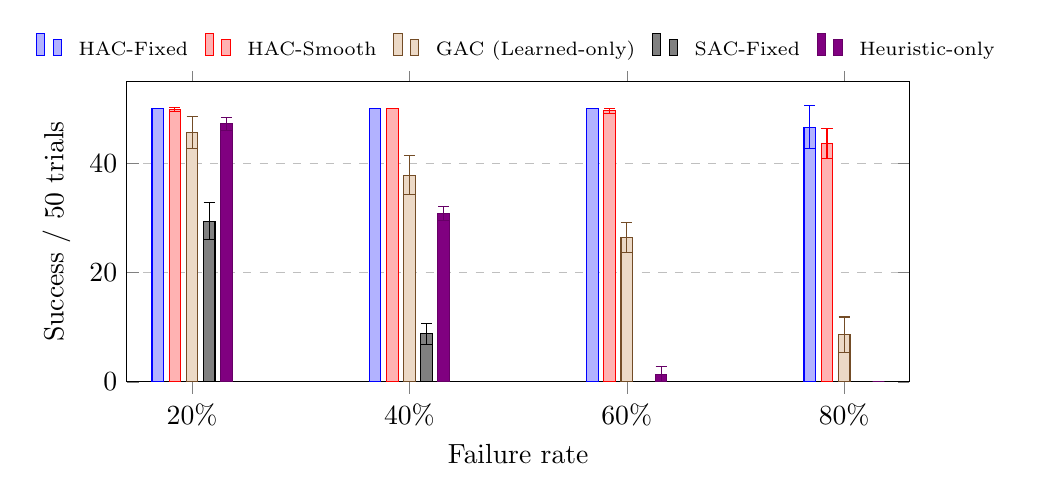
\begin{tikzpicture}
\begin{axis}[
  ybar, bar width=4.2pt,
  width=0.95\linewidth, height=5.4cm,
  ylabel={Success / 50 trials},
  xlabel={Failure rate},
  symbolic x coords={20\%,40\%,60\%,80\%},
  xtick=data,
  ymin=0, ymax=55,
  legend style={font=\scriptsize, draw=none, at={(0.5,1.18)}, anchor=north, legend columns=5, column sep=4pt},
  ymajorgrids=true, grid style=dashed,
  error bars/y dir=both, error bars/y explicit,
]
\addplot+[error bars/.cd, y dir=both, y explicit] coordinates {
  (20\%,50.0) +- (0,0.0) (40\%,50.0) +- (0,0.0) (60\%,50.0) +- (0,0.0) (80\%,46.6) +- (0,3.93)
};
\addplot+[error bars/.cd, y dir=both, y explicit] coordinates {
  (20\%,49.8) +- (0,0.4) (40\%,50.0) +- (0,0.0) (60\%,49.6) +- (0,0.49) (80\%,43.6) +- (0,2.80)
};
\addplot+[error bars/.cd, y dir=both, y explicit] coordinates {
  (20\%,45.6) +- (0,2.94) (40\%,37.8) +- (0,3.54) (60\%,26.4) +- (0,2.80) (80\%,8.6) +- (0,3.26)
};
\addplot+[error bars/.cd, y dir=both, y explicit] coordinates {
  (20\%,29.4) +- (0,3.38) (40\%,8.8) +- (0,1.94) (60\%,0.0) +- (0,0.0) (80\%,0.0) +- (0,0.0)
};
\addplot+[error bars/.cd, y dir=both, y explicit] coordinates {
  (20\%,47.2) +- (0,1.17) (40\%,30.8) +- (0,1.33) (60\%,1.4) +- (0,1.36) (80\%,0.0) +- (0,0.0)
};
\legend{HAC-Fixed,HAC-Smooth,GAC (Learned-only),SAC-Fixed,Heuristic-only}
\end{axis}
\end{tikzpicture}
\caption{Connectivity recovery success count (out of 50 trials) across node failure rates under random deployment (mean $\pm$ std over 5 seeds). Both HAC-Fixed and HAC-Smooth sustain high recovery rates across all failure regimes.}
\label{fig:success-random}
\end{figure}

\begin{table}[t]
\centering
\caption{Main benchmark results under uniform deployment (mean $\pm$ std over 5 seeds, 50 trials per seed). Here $^*$ denotes conditional averages over $<2/50$ successful trials (survivorship bias on trivial initial draws).}
\label{tab:main-uniform}
\scriptsize
\begin{tabular}{@{}llcccc@{}}
\toprule
Architecture & Failure & Success/50 $\uparrow$ & REC $\downarrow$ & COV $\uparrow$ & Runtime (s) $\downarrow$ \\
\midrule
\multirow{4}{*}{HAC-Fixed $(50/50)$}
 & 20\% & $50.0\pm0.0$ & $0.005\pm0.001$ & $1.000\pm0.000$ & $0.238\pm0.015$ \\
 & 40\% & $50.0\pm0.0$ & $0.040\pm0.004$ & $0.998\pm0.000$ & $0.269\pm0.027$ \\
 & 60\% & $50.0\pm0.0$ & $0.249\pm0.023$ & $0.960\pm0.004$ & $0.649\pm0.038$ \\
 & \textbf{80\%} & $\mathbf{49.4\pm0.8}$ & $\mathbf{0.643\pm0.026}$ & $\mathbf{0.609\pm0.004}$ & $\mathbf{1.208\pm0.059}$ \\
\midrule
\multirow{4}{*}{HAC-Smooth $(5, 0.7)$}
 & 20\% & $50.0\pm0.0$ & $0.005\pm0.001$ & $1.000\pm0.000$ & $0.233\pm0.012$ \\
 & 40\% & $50.0\pm0.0$ & $0.039\pm0.004$ & $0.998\pm0.000$ & $0.255\pm0.017$ \\
 & 60\% & $50.0\pm0.0$ & $0.252\pm0.019$ & $0.967\pm0.001$ & $0.633\pm0.040$ \\
 & \textbf{80\%} & $47.8\pm1.3$ & $0.665\pm0.040$ & $0.604\pm0.007$ & $1.262\pm0.098$ \\
\midrule
\multirow{4}{*}{GAC (Learned-only)}
 & 20\% & $49.6\pm0.5$ & $0.023\pm0.015$ & $0.988\pm0.009$ & $0.388\pm0.115$ \\
 & 40\% & $48.4\pm1.0$ & $0.211\pm0.014$ & $0.892\pm0.012$ & $1.016\pm0.095$ \\
 & 60\% & $36.4\pm3.3$ & $0.620\pm0.068$ & $0.569\pm0.048$ & $2.065\pm0.118$ \\
 & 80\% & $11.2\pm3.7$ & $0.839\pm0.039$ & $0.344\pm0.019$ & $1.937\pm0.099$ \\
\midrule
\multirow{4}{*}{SAC-Fixed (Subnet Rigid)}
 & 20\% & $48.8\pm1.2$ & $0.007\pm0.007$ & $0.999\pm0.001$ & $0.341\pm0.111$ \\
 & 40\% & $31.4\pm3.3$ & $0.161\pm0.013$ & $0.959\pm0.007$ & $1.492\pm0.266$ \\
 & 60\% & $0.2\pm0.4$  & $0.003\pm0.000^*$ & $0.964\pm0.000^*$ & $2.212\pm0.145$ \\
 & 80\% & $0.0\pm0.0$  & n/a & n/a & $1.851\pm0.155$ \\
\midrule
\multirow{4}{*}{Heuristic-only}
 & 20\% & $49.8\pm0.4$ & $0.006\pm0.002$ & $1.000\pm0.000$ & $0.228\pm0.022$ \\
 & 40\% & $44.0\pm1.3$ & $0.078\pm0.017$ & $0.998\pm0.000$ & $0.340\pm0.032$ \\
 & 60\% & $0.8\pm0.7$  & $0.110\pm0.081^*$ & $0.977\pm0.009^*$ & $0.776\pm0.057$ \\
 & 80\% & $0.0\pm0.0$  & n/a & n/a & $0.550\pm0.027$ \\
\bottomrule
\end{tabular}
\end{table}

\subsection{Comparison with Multipartite Subnetwork Architectures}
\label{sec:r2c-comparison}
\textbf{HAC-Fixed and HAC-Smooth retain $88.4\%$ to $91.2\%$ of the coverage reported by R2C under $80\%$ node failure despite omitting convex-hull boundary extraction, virtual multipartite edges, and spectral graph filtering.} Table~\ref{tab:r2c-comparison} compares HAC-Fixed against the published figures of R2C \citep{peng2026r2c}. At $20\%$ and $40\%$ failure rates, both methods achieve virtually identical coverage ($\ge 0.988$), with HAC-Fixed achieving faster recovery under uniform deployment ($\mathrm{REC}$ of $0.005$ vs.\ $0.037$ at $20\%$ failure and $0.040$ vs.\ $0.051$ at $40\%$ failure). Under the most severe $80\%$ failure regime, R2C's reported coverage exceeds that of HAC-Fixed by an absolute margin of $7.9\text{ pp}$ in random deployment ($0.681$ vs.\ $0.602$, or $6.5\text{ pp}$ vs.\ HAC-Smooth's $0.616$) and $5.9\text{ pp}$ in uniform deployment ($0.668$ vs.\ $0.609$), corresponding to a relative coverage retention of $88.4\%$ (random, $90.5\%$ for HAC-Smooth) and $91.2\%$ (uniform). Considering that R2C relies on Quickhull boundary extraction, multipartite cross-subnetwork edge construction, and an $8$-layer, $512$-dimensional spectral GCN, whereas HAC uses a single global $4$-layer, $128$-dimensional GCN, these results confirm that the primary resilience gain stems from coupling a local virtual-force prior with a global node-level learned policy rather than complex subnetwork partitioning.

\begin{table}[t]
\centering
\caption{Comparison between HAC-Fixed and published numbers of R2C \citep{peng2026r2c}. Lower $\mathrm{REC}\downarrow$ and higher $\mathrm{COV}\uparrow$ indicate superior recovery speed and spatial coverage.}
\label{tab:r2c-comparison}
\small
\begin{tabular}{@{}lcccccccc@{}}
\toprule
 & \multicolumn{4}{c}{Random Deployment} & \multicolumn{4}{c}{Uniform Deployment} \\
\cmidrule(lr){2-5}\cmidrule(lr){6-9}
Failure & \multicolumn{2}{c}{R2C \citep{peng2026r2c}} & \multicolumn{2}{c}{HAC-Fixed} & \multicolumn{2}{c}{R2C \citep{peng2026r2c}} & \multicolumn{2}{c}{HAC-Fixed} \\
\cmidrule(lr){2-3}\cmidrule(lr){4-5}\cmidrule(lr){6-7}\cmidrule(lr){8-9}
Rate & REC$\downarrow$ & COV$\uparrow$ & REC$\downarrow$ & COV$\uparrow$ & REC$\downarrow$ & COV$\uparrow$ & REC$\downarrow$ & COV$\uparrow$ \\
\midrule
20\% & 0.023 & 0.996 & 0.051 & 0.997 & 0.037 & 1.000 & 0.005 & 1.000 \\
40\% & 0.070 & 0.989 & 0.134 & 0.988 & 0.051 & 0.999 & 0.040 & 0.998 \\
60\% & 0.204 & 0.951 & 0.331 & 0.928 & 0.181 & 0.978 & 0.249 & 0.960 \\
80\% & 0.625 & \textbf{0.681} & 0.696 & \textbf{0.602} & 0.617 & \textbf{0.668} & 0.643 & \textbf{0.609} \\
\bottomrule
\end{tabular}
\end{table}

\subsection{Topology Quality and Anti-Clustering Analysis}
\textbf{HAC-Fixed and HAC-Smooth completely eliminate the GNN spatial-collapse failure mode while sustaining high topological reconnection.} Figure~\ref{fig:and-random} plots the five-seed post-recovery average node degree ($\mathrm{AND}$) across failure rates under random deployment. Whereas the purely learned GAC baseline exhibits inflated node degrees ($\mathrm{AND}$ rising to $10.12$ at $40\%$ failure and $9.27$ at $60\%$ failure) caused by inward GNN aggregation bias, HAC-Fixed and HAC-Smooth track the low, monotonically decreasing degree profile of Heuristic-only and SAC-Fixed ($\mathrm{AND}$ declining smoothly from $6.73$ and $6.63$ at $20\%$ failure to $2.58$ and $2.48$ at $80\%$ failure). Velocity-level fusion with the buffered virtual-force field preserves uniform spatial dispersion without sacrificing global reconnection reach.

\begin{figure}[t]
\centering
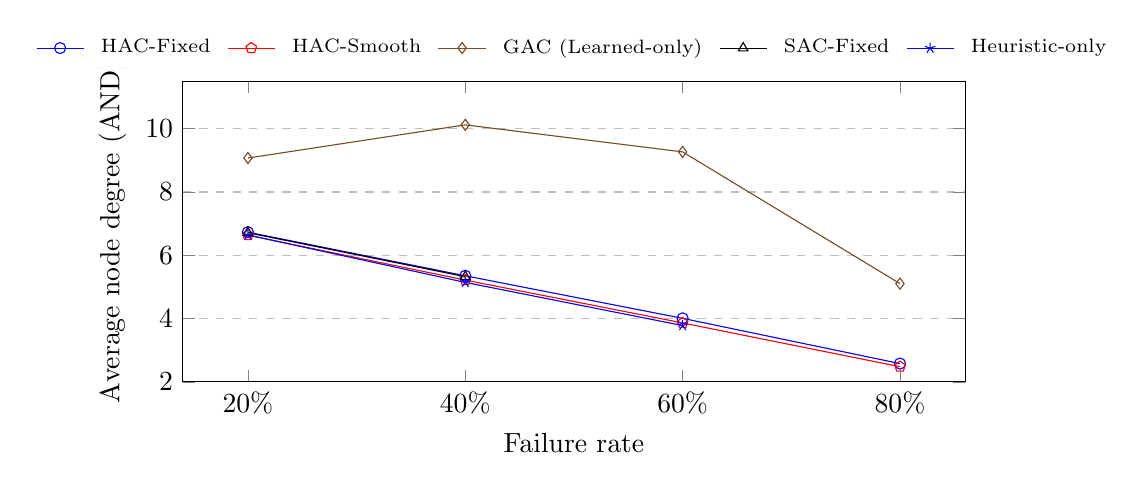
\begin{tikzpicture}
\begin{axis}[
  width=0.95\linewidth, height=5.4cm,
  xlabel={Failure rate}, ylabel={Average node degree (AND)},
  symbolic x coords={20\%,40\%,60\%,80\%},
  xtick=data,
  ymin=2, ymax=11.5,
  legend style={font=\scriptsize, draw=none, at={(0.5,1.18)}, anchor=north, legend columns=5, column sep=4pt},
  ymajorgrids=true, grid style=dashed,
]
\addplot+[mark=o] coordinates {(20\%,6.729) (40\%,5.352) (60\%,4.007) (80\%,2.578)};
\addplot+[mark=pentagon] coordinates {(20\%,6.634) (40\%,5.216) (60\%,3.862) (80\%,2.479)};
\addplot+[mark=diamond] coordinates {(20\%,9.073) (40\%,10.121) (60\%,9.267) (80\%,5.104)};
\addplot+[mark=triangle] coordinates {(20\%,6.713) (40\%,5.324) (60\%,{nan}) (80\%,{nan})};
\addplot+[mark=star] coordinates {(20\%,6.643) (40\%,5.142) (60\%,3.779) (80\%,{nan})};
\legend{HAC-Fixed,HAC-Smooth,GAC (Learned-only),SAC-Fixed,Heuristic-only}
\end{axis}
\end{tikzpicture}
\caption{Average node degree (AND) across failure rates under random deployment (5-seed mean). HAC-Fixed and HAC-Smooth avoid the high-degree spatial collapse of GAC while maintaining the highest recovery success rates.}
\label{fig:and-random}
\end{figure}

\subsection{Five-Seed Adaptive Fusion Schedule Sweep}
\label{sec:adaptive-ablation}
\textbf{Across five random seeds, reducing the transition slope $k$ monotonically improves $80\%$-failure recovery at every midpoint $s_0$, with the smooth schedule $(k=5, s_0=0.7)$ restoring near-optimal robustness across both deployments.} Table~\ref{tab:schedule-sweep} reports the five-seed schedule sweep across slope $k \in \{5, 10, 30\}$ and midpoint $s_0 \in \{0.125, 0.5, 0.7\}$ under random deployment. At $s_0 = 0.125$, reducing slope from $k=30$ to $k=10$ increases $80\%$-failure recovery from $14.2 \pm 4.3$ to $18.4 \pm 5.0$ and raises coverage from $0.413$ to $0.462$. At $s_0 = 0.5$, reducing slope from $k=30$ to $k=10$ boosts $80\%$-failure recovery nearly sixfold from $5.2 \pm 1.3$ to $29.6 \pm 4.5$ while cutting recovery time from $\mathrm{REC} = 0.855$ to $0.673$, directly confirming Proposition~\ref{prop:neutral-renorm}: under $(30, 0.5)$, $w_T(0; T) \approx 3 \times 10^{-7}$ suppresses neutral-zone global motion during the first half of the episode before abruptly extinguishing $w_E(t; T)$ in the second half. Widening the transition window further to $(k=5, s_0=0.7)$ satisfies both conditions of Proposition~\ref{prop:neutral-renorm} and reaches $43.6 \pm 2.8$ successes with $\mathrm{COV} = 0.616 \pm 0.006$ and $\mathrm{AND} = 2.479 \pm 0.058$ in random deployment, and $47.8 \pm 1.3$ successes with $\mathrm{COV} = 0.604 \pm 0.007$ in uniform deployment.

\begin{table}[t]
\centering
\caption{Five-seed adaptive fusion schedule sweep across slope $k$ and midpoint $s_0$ under random deployment (mean $\pm$ std over 5 seeds, 50 trials per seed). At every midpoint $s_0$, gentler slopes (smaller $k$) strictly improve $80\%$-failure recovery and coverage.}
\label{tab:schedule-sweep}
\scriptsize
\setlength{\tabcolsep}{3.2pt}
\begin{tabular}{@{}lccccccc@{}}
\toprule
 & \multicolumn{4}{c}{Success / 50 Trials $\uparrow$} & \multicolumn{3}{c}{Metrics at $80\%$ Failure} \\
\cmidrule(lr){2-5}\cmidrule(lr){6-8}
Schedule $(k, s_0)$ & 20\% & 40\% & 60\% & 80\% & REC $\downarrow$ & COV $\uparrow$ & AND \\
\midrule
Steep Early $(30, 0.125)$    & $49.4\pm0.5$ & $47.2\pm1.6$ & $41.0\pm3.3$ & $14.2\pm4.3$ & $0.796\pm0.032$ & $0.413\pm0.032$ & $4.114\pm0.296$ \\
Moderate Early $(10, 0.125)$ & $49.8\pm0.4$ & $49.4\pm0.8$ & $46.0\pm2.2$ & $18.4\pm5.0$ & $0.746\pm0.050$ & $0.462\pm0.036$ & $3.426\pm0.318$ \\
Steep Mid $(30, 0.5)$        & $49.8\pm0.4$ & $49.6\pm0.5$ & $42.8\pm0.7$ & $5.2\pm1.3$  & $0.855\pm0.037$ & $0.516\pm0.020$ & $2.604\pm0.152$ \\
Moderate Mid $(10, 0.5)$     & $50.0\pm0.0$ & $50.0\pm0.0$ & $49.8\pm0.4$ & $29.6\pm4.5$ & $\mathbf{0.673\pm0.016}$ & $0.571\pm0.022$ & $2.579\pm0.075$ \\
\textbf{HAC-Smooth $(5, 0.7)$} & $49.8\pm0.4$ & $50.0\pm0.0$ & $49.6\pm0.5$ & $43.6\pm2.8$ & $0.684\pm0.020$ & $\mathbf{0.616\pm0.006}$ & $\mathbf{2.479\pm0.058}$ \\
\textbf{HAC-Fixed $(50/50)$} & $\mathbf{50.0\pm0.0}$ & $\mathbf{50.0\pm0.0}$ & $\mathbf{50.0\pm0.0}$ & $\mathbf{46.6\pm3.9}$ & $0.696\pm0.048$ & $0.602\pm0.009$ & $2.578\pm0.027$ \\
\bottomrule
\end{tabular}
\end{table}

\subsection{Decoupled Training vs.\ Inference Schedule Matrix}
\label{sec:decouple-ablation}
\textbf{Cross-evaluating policies across all $3 \times 3$ pairings of training and evaluation schedules falsifies the training-corruption hypothesis and proves that steep-schedule collapse is strictly an inference-time handover phenomenon.} Table~\ref{tab:decouple-matrix} presents the five-seed $3 \times 3$ decoupled matrix crossing $w_T^{\mathrm{train}} \in \{\text{Fixed}, \text{Smooth } (5, 0.7), \text{Steep } (30, 0.125)\}$ with $w_T^{\mathrm{eval}} \in \{\text{Fixed}, \text{Smooth } (5, 0.7), \text{Steep } (30, 0.125)\}$ under random deployment at $60\%$ and $80\%$ failure. Two decisive findings emerge:
\begin{enumerate}[nosep]
  \item \textbf{Steep training does not impair the learned policy representation:} Models trained under the steep schedule ($w_T^{\mathrm{train}} = \text{Steep}$) achieve $46.6 \pm 0.5$ successes when evaluated with Fixed weights and $46.4 \pm 0.5$ successes when evaluated with Smooth weights at $80\%$ failure, accompanied by the highest coverage ($0.622 \pm 0.004$ and $0.624 \pm 0.003$) and lowest cross-seed variance ($\pm 0.5$ trials) in the entire study. Because training rollouts span $T_{\mathrm{train}} = 40$ steps, strong gradient supervision during early-to-mid rollout steps suffices to train a highly accurate global direction field $\pi_\theta$.
  \item \textbf{Steep evaluation collapses recovery regardless of how the policy was trained:} Evaluating under $w_T^{\mathrm{eval}} = \text{Steep}$ causes $80\%$-failure recovery to plummet to $9.8 \pm 3.8$ (for Fixed-trained policies), $12.0 \pm 4.6$ (for Smooth-trained policies), and $14.2 \pm 4.3$ (for Steep-trained policies), while coverage drops by $18$ to $21\text{ pp}$ (down to $0.410$--$0.439$) and node clustering spikes ($\mathrm{AND}$ rising from $\approx 2.48$ to $3.83$--$4.11$). Over the $400$-step inference horizon, driving $w_E^{\mathrm{eval}}(t; T) \to 0$ removes the heuristic link-retention barrier (Propositions~\ref{prop:monotonicity} and~\ref{prop:neutral-renorm}), causing the learned policy to over-cluster local nodes and stall before bridging distant components.
\end{enumerate}

\begin{table}[t]
\centering
\caption{Five-seed $3 \times 3$ decoupled training-versus-evaluation schedule matrix under random deployment (mean $\pm$ std over 5 seeds, 50 trials per seed). Collapse occurs exclusively when the \emph{evaluation} schedule is Steep ($w_T^{\mathrm{eval}} = \text{Steep}$), whereas policies trained under Steep scheduling perform excellently when evaluated under Fixed or Smooth schedules.}
\label{tab:decouple-matrix}
\scriptsize
\begin{tabular}{@{}llccccc@{}}
\toprule
Training & Evaluation & \multicolumn{2}{c}{Success / 50 $\uparrow$} & \multicolumn{3}{c}{Metrics at $80\%$ Failure} \\
\cmidrule(lr){3-4}\cmidrule(lr){5-7}
Schedule $w_T^{\mathrm{train}}$ & Schedule $w_T^{\mathrm{eval}}$ & 60\% Failure & 80\% Failure & REC $\downarrow$ & COV $\uparrow$ & AND \\
\midrule
\multirow{3}{*}{Fixed $(50/50)$}
 & Fixed $(50/50)$        & $50.0\pm0.0$ & $\mathbf{46.6\pm3.9}$ & $0.696\pm0.048$ & $0.602\pm0.009$ & $2.578\pm0.027$ \\
 & Smooth $(5, 0.7)$      & $49.2\pm0.7$ & $42.6\pm5.0$          & $0.702\pm0.042$ & $0.613\pm0.008$ & $2.483\pm0.026$ \\
 & Steep $(30, 0.125)$    & $38.4\pm3.4$ & $9.8\pm3.8$           & $0.768\pm0.070$ & $0.439\pm0.054$ & $3.828\pm0.508$ \\
\midrule
\multirow{3}{*}{Smooth $(5, 0.7)$}
 & Fixed $(50/50)$        & $50.0\pm0.0$ & $\mathbf{47.4\pm1.9}$ & $\mathbf{0.674\pm0.027}$ & $0.602\pm0.005$ & $2.580\pm0.026$ \\
 & Smooth $(5, 0.7)$      & $49.6\pm0.5$ & $43.6\pm2.8$          & $0.684\pm0.020$ & $0.616\pm0.006$ & $2.479\pm0.058$ \\
 & Steep $(30, 0.125)$    & $38.2\pm5.3$ & $12.0\pm4.6$          & $0.797\pm0.037$ & $0.410\pm0.027$ & $4.057\pm0.220$ \\
\midrule
\multirow{3}{*}{Steep $(30, 0.125)$}
 & Fixed $(50/50)$        & $49.4\pm0.5$ & $\mathbf{46.6\pm0.5}$ & $0.679\pm0.023$ & $0.622\pm0.004$ & $2.509\pm0.048$ \\
 & Smooth $(5, 0.7)$      & $49.2\pm0.7$ & $\mathbf{46.4\pm0.5}$ & $0.706\pm0.018$ & $\mathbf{0.624\pm0.003}$ & $\mathbf{2.474\pm0.043}$ \\
 & Steep $(30, 0.125)$    & $41.0\pm3.3$ & $14.2\pm4.3$          & $0.796\pm0.032$ & $0.413\pm0.032$ & $4.114\pm0.296$ \\
\bottomrule
\end{tabular}
\end{table}

\subsection{Granularity Substitution Counter-Experiment (HSC)}
\label{sec:hsc}
\textbf{Replacing HAC's node-level global GCN with a subnetwork-level rigid-translation GCN (HSC) causes deterministic recovery collapse at $80\%$ failure across all five seeds that schedule smoothing cannot rescue.} To verify whether smooth scheduling can compensate for restricted spatial expressiveness, we evaluate HSC across five random seeds under both deployments (Table~\ref{tab:hsc}). While smoothing the schedule from $(30, 0.125)$ to $(5, 0.7)$ improves HSC's recovery at $60\%$ failure from $12.2 \pm 3.7$ to $40.8 \pm 1.5$ (random) and from $13.0 \pm 4.9$ to $45.0 \pm 2.8$ (uniform), all HSC variants collapse to $0.0 \pm 0.0$--$0.4 \pm 0.5$ out of $50$ at $80\%$ failure. When a policy's output space is restricted to rigid component translation, no fusion schedule can supply the node-level degrees of freedom required to bridge severe multi-directional fragmentation.

\begin{table}[t]
\centering
\caption{Five-seed granularity substitution counter-experiment with HSC (heuristic branch fused with subnetwork-level rigid translation, Success/50, mean $\pm$ std over 5 seeds). Unlike node-level HAC, HSC collapses at $80\%$ failure regardless of schedule smoothness.}
\label{tab:hsc}
\scriptsize
\setlength{\tabcolsep}{4.2pt}
\begin{tabular}{@{}lcccccccc@{}}
\toprule
 & \multicolumn{4}{c}{Random Deployment (Success/50 $\uparrow$)} & \multicolumn{4}{c}{Uniform Deployment (Success/50 $\uparrow$)} \\
\cmidrule(lr){2-5}\cmidrule(lr){6-9}
Variant & 20\% & 40\% & 60\% & 80\% & 20\% & 40\% & 60\% & 80\% \\
\midrule
HSC-Fixed $(50/50)$     & $49.2\pm0.7$ & $47.6\pm1.5$ & $38.0\pm2.7$ & $0.4\pm0.5$ & $50.0\pm0.0$ & $49.6\pm0.5$ & $46.4\pm1.4$ & $0.2\pm0.4$ \\
HSC-Steep $(30, 0.125)$ & $50.0\pm0.0$ & $47.2\pm1.5$ & $12.2\pm3.7$ & $0.0\pm0.0$ & $50.0\pm0.0$ & $49.4\pm0.5$ & $13.0\pm4.9$ & $0.0\pm0.0$ \\
HSC-Smooth $(5, 0.7)$   & $50.0\pm0.0$ & $49.2\pm0.7$ & $40.8\pm1.5$ & $0.0\pm0.0$ & $50.0\pm0.0$ & $49.8\pm0.4$ & $45.0\pm2.8$ & $0.0\pm0.0$ \\
\bottomrule
\end{tabular}
\end{table}

\section{Discussion and Conclusion}
\label{sec:discussion}
\label{sec:conclusion}

\subsection{Design Insights and Engineering Guidelines}
\textbf{Velocity-level hybrid controllers succeed because the heuristic and learned branches resolve orthogonal failure modes through state-triggered neutral-zone renormalization.} The virtual-force branch guarantees local link retention and inter-UAV spacing within connected components while leaving an interior neutral band $[d_l, d_u]$ where local forces vanish. Because unit-speed velocity renormalization amplifies the global GCN command whenever local forces equilibrate inside this neutral zone, the swarm translates at full speed toward disconnected components without sacrificing link-retention priority at component boundaries. Our decoupled cross-evaluation matrix demonstrates that maintaining a non-vanishing heuristic weight throughout inference is essential, and that pairing an aggressive training schedule with a conservative fixed or smooth evaluation schedule yields the highest post-recovery coverage and lowest cross-seed variance.

\textbf{Practitioners building hybrid swarm recovery systems should prioritize node-level actuation authority and persistent inference-time heuristic damping over complex geometric partitioning.} Comparing node-level HAC against subnetwork-level HSC establishes that temporal schedule tuning cannot substitute for spatial degrees of freedom when severe node loss shatters the network into scattered singletons. Constant equal weighting or wide-window smooth gating provides a robust, zero-tuning default that avoids the inference-time collapse of sharp stage switches.

\subsection{Limitations and Future Directions}
\textbf{Incorporating lightweight node-level boundary features and extending differentiable training horizons offer promising directions for closing the remaining coverage margin against multipartite architectures.} While HAC retains roughly $90\%$ of the coverage reported by R2C under extreme node failure without Quickhull boundary extraction or multipartite virtual edges, augmenting node features with local anisotropy indicators or deeper spectral convolutions could close the remaining single-digit percentage-point coverage margin while preserving node-level simplicity. Furthermore, extending differentiable rollout horizons beyond $40$ steps via truncated backpropagation through time and evaluating physical wind disturbances and second-order flight dynamics will further strengthen real-world deployment readiness.

\subsection{Conclusion}
This paper systematically disentangled the roles of decision paradigm, spatial reasoning granularity, and temporal fusion scheduling in self-healing UAV swarm connectivity recovery. Through five-seed benchmarks across random and uniform deployments, we showed that Hybrid Adaptive Convolution (HAC), which fuses a parameter-free buffered virtual-force heuristic with a single global node-level GCN at the velocity level, outperforms purely heuristic, purely learned, and subnetwork-level rigid baselines while retaining the vast majority of the coverage reported by complex multipartite architectures without boundary-hull extraction. Through theoretical analysis of link-retention barriers and neutral-zone velocity renormalization alongside a five-seed $3 \times 3$ decoupled training-versus-evaluation schedule matrix, we falsified the hypothesis that steep adaptive schedules corrupt policy learning during training and proved instead that premature inference-time handover extinguishes the heuristic link-retention barrier during long-horizon rollouts. Combined with granularity-substitution counter-experiments on HSC and our cardinality-invariant connectivity surrogate loss, these findings provide a rigorous, reproducible foundation for designing simple and resilient hybrid swarm controllers.

\bibliographystyle{plainnat}
\bibliography{references}

\appendix

\section{Methodological Verification and Reproducibility Log}
\label{app:deviations}

To ensure full reproducibility and clarify experimental design choices relative to prior literature \citep{peng2026r2c}, we document all simulation specifications and numerical verifications below:
\begin{itemize}[nosep]
  \item \textbf{Failure-node sampling:} Failed UAVs at ratios $\{20\%, 40\%, 60\%, 80\%\}$ are sampled uniformly at random without replacement from the initial deployed swarm.
  \item \textbf{Cardinality-invariant connectivity loss verification:} As derived in Eq.~\eqref{eq:conn-loss}, omitting the $-\log(n_i n_j)$ normalization term in a log-sum-exp soft-minimum surrogate introduces a severe component-size bias. On a controlled synthetic benchmark featuring two disconnected components separated by an identical true minimum distance ($\approx 100$ to $108\,\mathrm{m}$) under two cardinality configurations ($3\times3$ nodes vs.\ $30\times30$ nodes), the unnormalized log-sum-exp estimator returned $2.85$ for the $3\times3$ pair and $-230.58$ for the $30\times30$ pair. In contrast, our cardinality-invariant estimator in Eq.~\eqref{eq:conn-loss} returned $112.71$ and $109.54$, respectively, accurately tracking the true geometric separation regardless of cluster size.
  \item \textbf{Boundary buffer specification:} The arena boundary repulsion buffer is set to $d_e = 0.15 R_c = 18\,\mathrm{m}$, matching the scale of the inter-UAV equilibrium band $d_u - d_l = 0.1 R_c = 12\,\mathrm{m}$.
  \item \textbf{Differentiable rollout horizon:} Training uses $T_{\mathrm{train}} = 40$ differentiable rollout steps per epoch for backpropagation-through-time tractability, while evaluation runs for the full horizon $T = 400$ steps.
  \item \textbf{Grid-based coverage evaluation:} Swarm coverage $C_{\mathrm{cov}}(t)$ is evaluated over a deterministic uniform grid at $5\,\mathrm{m}$ spatial resolution across the $1000 \times 1000\,\mathrm{m}^2$ arena.
  \item \textbf{Full-pipeline random seeding and auxiliary unprojected GAC logs:} Every five-seed experiment locks Python, NumPy, CPU PyTorch (\texttt{torch.manual\_seed}), and CUDA PyTorch (\texttt{torch.cuda.manual\_seed\_all}) generators prior to both network initialization and environment reset. In addition to the unit-norm projected GAC (Learned-only) baseline reported in the main tables from \texttt{summary\_multiseed\_all.csv}, we also evaluated an unprojected $\tanh$-scaled variant across five seeds, which achieved Success/50 of $49.0\pm0.6 \to 47.2\pm1.7 \to 42.8\pm3.7 \to 19.8\pm5.5$ and $\mathrm{COV}$ of $0.747\pm0.009 \to 0.614\pm0.021 \to 0.452\pm0.022 \to 0.310\pm0.009$ (with severe clustering $\mathrm{AND} = 13.68\pm0.28$ at $20\%$ failure under random deployment, and an unseeded single-run outlier of $\mathrm{COV}=0.830, \mathrm{AND}=11.87$), confirming that purely learned global GNNs suffer from spatial collapse and high initialization variance regardless of output projection.
\end{itemize}

\section{Full Hyperparameter Table}
\label{app:hyperparams}

\begin{table}[ht]
\centering
\caption{Hyperparameters shared across all evaluated architectures and five-seed training runs.}
\small
\begin{tabular}{@{}ll@{}}
\toprule
Parameter & Value \\
\midrule
Graph convolution layers $L$ & 4 \\
Hidden feature dimension & 128 \\
Global $k$-NN degree $k$ & 8 \\
Optimizer & Adam \\
Learning rate & $1\times10^{-3}$ \\
Gradient norm clipping threshold & 1.0 \\
Training epochs & 300 \\
Training rollout length $T_{\mathrm{train}}$ & 40 steps \\
Evaluation horizon $T$ & 400 steps \\
Independent random seeds per configuration & 5 seeds $\times$ 50 trials \\
Movement cost weight $\lambda$ & 0.01 \\
Heuristic decay rates $\alpha, \beta, \delta$ & 0.01 \\
Equilibrium buffer zone $[d_l, d_u]$ & $[0.8 R_c, 0.9 R_c]$ \\
Communication and coverage radii $R_c = R_{\mathrm{cov}}$ & $120\,\mathrm{m}$ \\
Maximum UAV speed $\hat{v}_{\max}$ & $1\,\mathrm{m/s}$ \\
Mission area $\mathcal{A} = [0, D_{\mathcal{A}}]^2$ & $1000\times1000\,\mathrm{m}^2$ ($D_{\mathcal{A}} = 1000\,\mathrm{m}$) \\
Random deployment initial UAV count & 200 \\
Uniform deployment initial UAV count & 196 ($14\times14$ grid) \\
\bottomrule
\end{tabular}
\end{table}

\section{Additional Five-Seed Topology Metrics for Uniform Deployment}
\label{app:additional}

Tables~\ref{tab:main-random} and~\ref{tab:main-uniform} in the main text report full Success/50, REC, COV, and Runtime statistics across all failure ratios. For completeness, the five-seed post-recovery average node degree ($\mathrm{AND}$, mean $\pm$ std) trajectories under uniform deployment across failure ratios $(20\% \to 40\% \to 60\% \to 80\%)$ from \texttt{summary\_multiseed\_all.csv} are:
\begin{itemize}[nosep]
  \item \textbf{HAC-Fixed $(50/50)$:} $5.723\pm0.011 \to 4.347\pm0.020 \to 3.298\pm0.038 \to 2.302\pm0.033$
  \item \textbf{HAC-Smooth $(5, 0.7)$:} $5.722\pm0.011 \to 4.333\pm0.023 \to 3.237\pm0.018 \to 2.278\pm0.033$
  \item \textbf{GAC (Learned-only):} $6.050\pm0.300 \to 6.158\pm0.248 \to 7.493\pm0.916 \to 4.730\pm0.549$
  \item \textbf{SAC-Fixed (Subnet Rigid):} $5.724\pm0.010 \to 4.379\pm0.035 \to 3.205\pm0.000^* \to \text{n/a}$
  \item \textbf{Heuristic-only:} $5.724\pm0.011 \to 4.358\pm0.020 \to 2.870\pm0.256^* \to \text{n/a}$
\end{itemize}
Consistent with the random-deployment analysis in Figure~\ref{fig:and-random}, both HAC-Fixed and HAC-Smooth maintain a low, monotonically decreasing node degree across all failure regimes under uniform deployment, whereas GAC exhibits pronounced mid-regime clustering ($\mathrm{AND} = 7.493 \pm 0.916$ at $60\%$ failure).

\section{Code and Reproducibility Artifacts}
\label{app:code}

The companion repository contains the complete simulation environment (\texttt{code/sim/}), heuristic virtual-force and global GCN model definitions (\texttt{code/models/}), differentiable rollout training and evaluation scripts (\texttt{code/scripts/}), shell scripts for multi-seed execution (\nolinkurl{run_full_multiseed_study.sh}), and aggregated five-seed CSV logs (\texttt{code/results/}) reproducing every table and figure in this manuscript.

\end{document}
